

Now, we will test the model that we have trained with our data that we have preporces, by taking the predict function into a while loop, asking the user for input,   output is either negative, neutral or positive.

 
\begin{lstlisting}[
                   language = python,
                   xleftmargin = 0.1cm,
                   framexleftmargin = 1em]
def predict(text, include_neutral=True):
    # Tokenize text
    x_test = pad_sequences(tokenizer.texts_to_sequences([text]), maxlen=MAX_SEQUENCE_LENGTH)
    # Predict
    score = model.predict([x_test])[0]
    # Decode sentiment
    label = decode_sentiment(score, include_neutral=include_neutral)

    return {"label": label, "score": float(score)}
 \end{lstlisting}
 
 The image below shows a demonstration of the process of our model:
\begin{center}
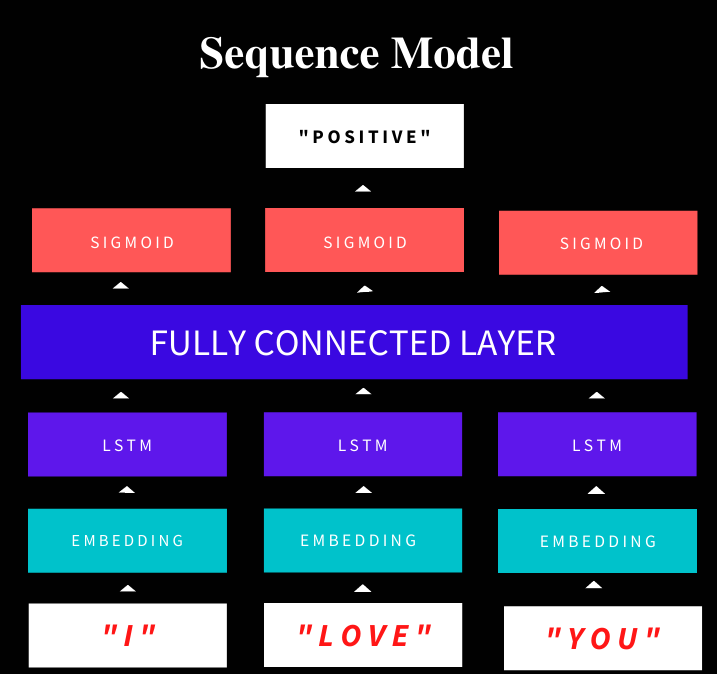
\includegraphics[scale=0.6]{SequenceModel.png}
\end{center}

